\documentclass[journal,12pt,twocolumn]{IEEEtran}
%
\usepackage[latin1]{inputenc}
\usepackage{setspace}
\usepackage{gensymb}
\doublespacing
\singlespacing

\usepackage{graphicx}
\usepackage{amssymb}
%\usepackage{relsize}
\usepackage[cmex10]{amsmath}
\usepackage{amsthm}
%\interdisplaylinepenalty=2500
%\savesymbol{iint}
%\usepackage{txfonts}
%\restoresymbol{TXF}{iint}
%\usepackage{wasysym}
\usepackage{amsthm}
%\usepackage{iithtlc}
\usepackage{mathrsfs}
\usepackage{txfonts}
\usepackage{stfloats}
\usepackage{bm}
\usepackage{cite}
\usepackage{cases}
\usepackage{subfig}
%\usepackage{xtab}
\usepackage{longtable}
\usepackage{multirow}
%\usepackage{algorithm}
%\usepackage{algpseudocode}
\usepackage{enumitem}
\usepackage{mathtools}
\usepackage{steinmetz}
\usepackage{tikz}
\usepackage{circuitikz}
\usepackage{verbatim}
\usepackage{tfrupee}
\usepackage[breaklinks=true]{hyperref}
%\usepackage{stmaryrd}
\usepackage{tkz-euclide} % loads  TikZ and tkz-base
%\usetkzobj{all}
\usetikzlibrary{calc,math}
\usepackage{listings}
    \usepackage{color}                                            %%
    \usepackage{array}                                            %%
    \usepackage{longtable}                                        %%
    \usepackage{calc}                                             %%
    \usepackage{multirow}                                         %%
    \usepackage{hhline}                                           %%
    \usepackage{ifthen}                                           %%
  %optionally (for landscape tables embedded in another document): %%
    \usepackage{lscape}     
\usepackage{multicol}
\usepackage{chngcntr}
%\usepackage{enumerate}
\usepackage{graphics}
%\usepackage{wasysym}
%\newcounter{MYtempeqncnt}
\DeclareMathOperator*{\Res}{Res}
%\renewcommand{\baselinestretch}{2}
\renewcommand\thesection{\arabic{section}}
\renewcommand\thesubsection{\thesection.\arabic{subsection}}
\renewcommand\thesubsubsection{\thesubsection.\arabic{subsubsection}}
\renewcommand{\theequation}{\thesection\arabic{equation}}
\renewcommand\thesectiondis{\arabic{section}}
\renewcommand\thesubsectiondis{\thesectiondis.\arabic{subsection}}
\renewcommand\thesubsubsectiondis{\thesubsectiondis.\arabic{subsubsection}}

% correct bad hyphenation here
\hyphenation{op-tical net-works semi-conduc-tor}
\def\inputGnumericTable{}                                 %%

\lstset{
%language=C,
frame=single, 
breaklines=true,
columns=fullflexible
}
%\lstset{
%language=tex,
%frame=single, 
%breaklines=true
%}

\begin{document}
%


\newtheorem{theorem}{Theorem}[section]
\newtheorem{problem}{Problem}
\newtheorem{proposition}{Proposition}[section]
\newtheorem{lemma}{Lemma}[section]
\newtheorem{corollary}[theorem]{Corollary}
\newtheorem{example}{Example}[section]
\newtheorem{definition}[problem]{Definition}
%\newtheorem{thm}{Theorem}[section] 
%\newtheorem{defn}[thm]{Definition}
%\newtheorem{algorithm}{Algorithm}[section]
%\newtheorem{cor}{Corollary}
\newcommand{\BEQA}{\begin{eqnarray}}
\newcommand{\EEQA}{\end{eqnarray}}
\newcommand{\define}{\stackrel{\triangle}{=}}
\bibliographystyle{IEEEtran}
%\bibliographystyle{ieeetr}
\providecommand{\mbf}{\mathbf}
\providecommand{\pr}[1]{\ensuremath{\Pr\left(#1\right)}}
\providecommand{\qfunc}[1]{\ensuremath{Q\left(#1\right)}}
\providecommand{\sbrak}[1]{\ensuremath{{}\left[#1\right]}}
\providecommand{\lsbrak}[1]{\ensuremath{{}\left[#1\right.}}
\providecommand{\rsbrak}[1]{\ensuremath{{}\left.#1\right]}}
\providecommand{\brak}[1]{\ensuremath{\left(#1\right)}}
\providecommand{\lbrak}[1]{\ensuremath{\left(#1\right.}}
\providecommand{\rbrak}[1]{\ensuremath{\left.#1\right)}}
\providecommand{\cbrak}[1]{\ensuremath{\left\{#1\right\}}}
\providecommand{\lcbrak}[1]{\ensuremath{\left\{#1\right.}}
\providecommand{\rcbrak}[1]{\ensuremath{\left.#1\right\}}}
\theoremstyle{remark}
\newtheorem{rem}{Remark}
\newcommand{\sgn}{\mathop{\mathrm{sgn}}}
\providecommand{\abs}[1]{\left\vert#1\right\vert}
\providecommand{\res}[1]{\Res\displaylimits_{#1}} 
\providecommand{\norm}[1]{\left\lVert#1\right\rVert}
%\providecommand{\norm}[1]{\lVert#1\rVert}
\providecommand{\mtx}[1]{\mathbf{#1}}
\providecommand{\mean}[1]{E\left[ #1 \right]}
\providecommand{\fourier}{\overset{\mathcal{F}}{ \rightleftharpoons}}
%\providecommand{\hilbert}{\overset{\mathcal{H}}{ \rightleftharpoons}}
\providecommand{\system}{\overset{\mathcal{H}}{ \longleftrightarrow}}
	%\newcommand{\solution}[2]{\textbf{Solution:}{#1}}
\newcommand{\solution}{\noindent \textbf{Solution: }}
\newcommand{\cosec}{\,\text{cosec}\,}
\providecommand{\dec}[2]{\ensuremath{\overset{#1}{\underset{#2}{\gtrless}}}}
\newcommand{\myvec}[1]{\ensuremath{\begin{pmatrix}#1\end{pmatrix}}}
\newcommand{\mydet}[1]{\ensuremath{\begin{vmatrix}#1\end{vmatrix}}}
%\numberwithin{equation}{section}
\numberwithin{equation}{subsection}
%\numberwithin{problem}{section}
%\numberwithin{definition}{section}
\makeatletter
\@addtoreset{figure}{problem}
\makeatother
\let\StandardTheFigure\thefigure
\let\vec\mathbf
%\renewcommand{\thefigure}{\theproblem.\arabic{figure}}
%\renewcommand{\thefigure}{\theproblem}
%\setlist[enumerate,1]{before=\renewcommand\theequation{\theenumi.\arabic{equation}}
%\counterwithin{equation}{enumi}
%\renewcommand{\theequation}{\arabic{subsection}.\arabic{equation}}
\def\putbox#1#2#3{\makebox[0in][l]{\makebox[#1][l]{}\raisebox{\baselineskip}[0in][0in]{\raisebox{#2}[0in][0in]{#3}}}}
     \def\rightbox#1{\makebox[0in][r]{#1}}
     \def\centbox#1{\makebox[0in]{#1}}
     \def\topbox#1{\raisebox{-\baselineskip}[0in][0in]{#1}}
     \def\midbox#1{\raisebox{-0.5\baselineskip}[0in][0in]{#1}}
\vspace{3cm}
\title{Linear Algebra}
\author{Mohit Singh}

\maketitle{}
\newpage
%\tableofcontents
\bigskip
\renewcommand{\thefigure}{\theenumi}
\renewcommand{\thetable}{\theenumi}

\begin{abstract}
This document provides the solution to the problem no. 7 of each section under  linear algebra. The figures are constructed using python.
\end{abstract}

\noindent This documentation can be downloaded from 
%
\begin{lstlisting}
svn co https://github.com/mohit-singh-9/Summer-2020/tree/master/geometry/linear_algebra.git
\end{lstlisting}
%
%and latex-tikz codes from 
%\begin{lstlisting}
%math/codes/tri_sss.py
%\end{lstlisting}

\section{TRIANGLE EXERCISE}
\subsection{Problem}
Sketch the circles with
\begin{align}
\brak{a}centre \myvec{0\\2}, radius 2
\\
\brak{b}centre \myvec{-2\\32}, radius 4
\\
\brak{c}centre \myvec{\frac{1}{2}\\\frac{1}{4}}, radius \frac{1}{12}
\\
\brak{d}centre \myvec{1\\1}, radius \sqrt{2}
\\
\brak{e}centre \myvec{-a\\-b}, radius \sqrt{a^2-b^2}
\end{align}

\subsection{Solution}
From theory, we understand that using dot product we can find the angle between the lines 
\begin{enumerate}
	\item 
	\begin{align}\label{eq:solutions/line_plane/74/codes:5}
		\frac{x-2}{2} = \frac{y-1}{5} &= \frac{z+3}{-3}, 
	\end{align}
	\begin{align}\label{eq:solutions/line_plane/74/codes:6}
		\frac{x+2}{-1} = \frac{y-4}{8} &= \frac{z-5}{4} 
	\end{align}


The above symmetric equations \ref{eq:solutions/line_plane/74/codes:5}, \ref{eq:solutions/line_plane/74/codes:6} can be represented in the vector form as 
\begin{align}\label{eq:solutions/line_plane/74/codes7}
	\quad \vec{r_1} &= \myvec{2\\1\\-3} + \lambda_1\myvec{2\\5\\-3}
	\\
	\quad \vec{r_2} &= \myvec{-2\\4\\5} + \lambda_2\myvec{-1\\8\\4}
\end{align}

As we have to find the angle between the vectors, we will only be taking the direction vectors into consideration. The direction vectors are $\vec{u}$ = $\myvec{2\\5\\-3}$ and $\vec{v}$ = $\myvec{-1\\8\\4}$. We can find the corresponding magnitude values

\begin{align}\label{eq:solutions/line_plane/74/codes9}
	\norm{\vec{u}} =\sqrt{2^{2}+5^{2}+(-3)^{2}} =\sqrt{38}
\end{align}
\begin{align}\label{eq:solutions/line_plane/74/codes10}
	\norm{\vec{v}} =\sqrt{(-1)^{2}+8^{2}+4^{2}} =\sqrt{81}
\end{align}

Using \ref{eq:solutions/line_plane/74/codes4}, \ref{eq:solutions/line_plane/74/codes9}, \ref{eq:solutions/line_plane/74/codes10} we get
\begin{align}
	\theta = \cos ^{-1}\frac{\myvec{2\\5\\-3}^{T}\myvec{-1\\8\\4}}{(\sqrt{38})(\sqrt{81})} 
	\\
	\theta = \cos ^{-1}\frac{26}{55.4797}
	\\
	\theta = \cos ^{-1} (0.4686)
	\\
	\theta = 62.053\degree
\end{align}

Therefore, the angle between the two lines is $62.053\degree$.See Fig. \ref{fig:solutions/line_plane/74/codesline_equation_1}

\begin{figure}
	\centering
	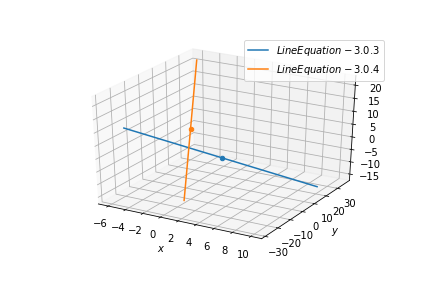
\includegraphics[width=\columnwidth]{./solutions/line_plane/74/codes/figs/Line_interest_1.png}
	\caption{Graph for equations \ref{eq:solutions/line_plane/74/codes7}}
	\label{fig:solutions/line_plane/74/codesline_equation_1}
\end{figure}


	\item 
	\begin{align}\label{eq:solutions/line_plane/74/codes12}
		\frac{x}{2} = \frac{y}{2} &= \frac{z}{1}, 
	\end{align}
	\begin{align}\label{eq:solutions/line_plane/74/codes13}
		\frac{x-5}{4} = \frac{y-2}{1} &= \frac{z-3}{8} 
	\end{align}



The above symmetric equations \ref{eq:solutions/line_plane/74/codes12}, \ref{eq:solutions/line_plane/74/codes13} can be represented in the vector form as 
\begin{align}\label{eq:solutions/line_plane/74/codes14}
	\quad \vec{r_1} &= \myvec{0\\0\\0} + \lambda_1\myvec{2\\2\\1}
	\\
	\quad \vec{r_2} &= \myvec{5\\2\\3} + \lambda_2\myvec{4\\1\\8}
\end{align}

As we have to find the angle between the vectors, we will only be taking the direction vectors into consideration. The direction vectors are $\vec{u}$ = $\myvec{2\\2\\1}$ and $\vec{v}$ = $\myvec{4\\1\\8}$. We can find the corresponding magnitude values

\begin{align}\label{eq:solutions/line_plane/74/codes16}
	\norm{\vec{u}} =\sqrt{2^{2}+2^{2}+1^{2}} =\sqrt{9}
\end{align}
\begin{align}\label{eq:solutions/line_plane/74/codes17}
	\norm{\vec{v}} =\sqrt{4^{2}+1^{2}+8^{2}} =\sqrt{81}
\end{align}

Using \ref{eq:solutions/line_plane/74/codes4}, \ref{eq:solutions/line_plane/74/codes16}, \ref{eq:solutions/line_plane/74/codes17} we get
\begin{align}
	\theta = \cos ^{-1}\frac{\myvec{2\\2\\1}^{T}\myvec{4\\1\\8}}{(\sqrt{9})(\sqrt{81})} 
	\\
	\theta = \cos ^{-1}\frac{18}{27.00}
	\\
	\theta = \cos ^{-1} (0.667)
	\\
	\theta = 48.189\degree
\end{align}

Therefore, the angle between the two lines is $48.189\degree$. See Fig. \ref{fig:solutions/line_plane/74/codesline_equation_2}


\begin{figure}
	\centering
	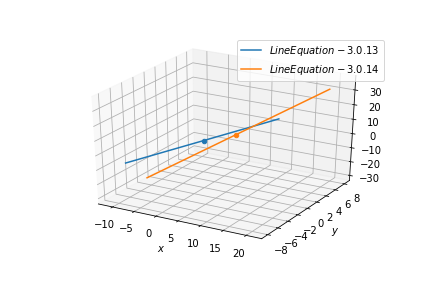
\includegraphics[width=\columnwidth]{./solutions/line_plane/74/codes/figs/Line_interest_2.png}
	\caption{Graph for equations \ref{eq:solutions/line_plane/74/codes14}}
	\label{fig:solutions/line_plane/74/codesline_equation_2}
\end{figure}
\end{enumerate}

    


\section{QUADRILATERAL EXERCISE}
\subsection{Problem}
Sketch the circles with
\begin{align}
\brak{a}centre \myvec{0\\2}, radius 2
\\
\brak{b}centre \myvec{-2\\32}, radius 4
\\
\brak{c}centre \myvec{\frac{1}{2}\\\frac{1}{4}}, radius \frac{1}{12}
\\
\brak{d}centre \myvec{1\\1}, radius \sqrt{2}
\\
\brak{e}centre \myvec{-a\\-b}, radius \sqrt{a^2-b^2}
\end{align}

\subsection{Solution}
\begin{align}
\myvec{1\\1} &= \sqrt{2}\myvec{\frac{1}{\sqrt{2}}\\ \frac{1}{\sqrt{2}}}
\\
&= \sqrt{2}\myvec{\cos 45\degree \\ \sin 45\degree}
\label{eq:3.4.7}
\end{align}
In the above, the modulus is $\norm{\myvec{1\\1}}=\sqrt{2}$ and the argument is $45 \degree$.
Similarly, 
\begin{align}
\myvec{1\\-1} &= \sqrt{2}\myvec{\cos 45\degree \\ -\sin 45\degree}
\\
\implies \myvec{1\\-1}^{-1} &= \frac{1}{\sqrt{2}}\myvec{\cos 45\degree \\ \sin 45\degree}
\end{align}
Using the matrix representation, 
\begin{align}
\frac{\myvec{1\\1}}{\myvec{1\\-1}} &= \myvec{\cos45\degree&-\sin45\degree\\\sin45\degree&\cos45\degree}
\nonumber \\
&\quad \times  \myvec{\cos45\degree&-\sin45\degree\\\sin45\degree&\cos45\degree}
\myvec{1\\0}
\\
 &= \myvec{\cos 90\degree\\ \sin 90\degree}= 1 \phase{90\degree}\end{align}
%
In general, if
\begin{align}
\vec{z}_1 &= r_1\myvec{\cos\theta_1\\\sin\theta_1}, \vec{z}_2 = r_2\myvec{\cos\theta_2\\\sin\theta_2},
\\
\vec{z}_1\vec{z}_2 &= r_1r_2\myvec{\cos(\theta_1+\theta_2)\\\sin(\theta_1+\theta_2)}.
\end{align}
Similarly, from \eqref{eq:3.4.7},
\begin{align}
\frac{1}{\myvec{1\\1}} &= \frac{1}{\sqrt{2}}\myvec{\cos 45\degree \\ -\sin 45\degree}
\\
&= \frac{1}{\sqrt{2}}\phase{-45\degree}
\end{align}



\section{LINE EXERCISE}
\subsection{Matrix}
\subsubsection{Problem}
Sketch the circles with
\begin{align}
\brak{a}centre \myvec{0\\2}, radius 2
\\
\brak{b}centre \myvec{-2\\32}, radius 4
\\
\brak{c}centre \myvec{\frac{1}{2}\\\frac{1}{4}}, radius \frac{1}{12}
\\
\brak{d}centre \myvec{1\\1}, radius \sqrt{2}
\\
\brak{e}centre \myvec{-a\\-b}, radius \sqrt{a^2-b^2}
\end{align}

\subsubsection{Solution}
From theory, we understand that using dot product we can find the angle between the lines 
\begin{enumerate}
	\item 
	\begin{align}\label{eq:solutions/line_plane/74/codes:5}
		\frac{x-2}{2} = \frac{y-1}{5} &= \frac{z+3}{-3}, 
	\end{align}
	\begin{align}\label{eq:solutions/line_plane/74/codes:6}
		\frac{x+2}{-1} = \frac{y-4}{8} &= \frac{z-5}{4} 
	\end{align}


The above symmetric equations \ref{eq:solutions/line_plane/74/codes:5}, \ref{eq:solutions/line_plane/74/codes:6} can be represented in the vector form as 
\begin{align}\label{eq:solutions/line_plane/74/codes7}
	\quad \vec{r_1} &= \myvec{2\\1\\-3} + \lambda_1\myvec{2\\5\\-3}
	\\
	\quad \vec{r_2} &= \myvec{-2\\4\\5} + \lambda_2\myvec{-1\\8\\4}
\end{align}

As we have to find the angle between the vectors, we will only be taking the direction vectors into consideration. The direction vectors are $\vec{u}$ = $\myvec{2\\5\\-3}$ and $\vec{v}$ = $\myvec{-1\\8\\4}$. We can find the corresponding magnitude values

\begin{align}\label{eq:solutions/line_plane/74/codes9}
	\norm{\vec{u}} =\sqrt{2^{2}+5^{2}+(-3)^{2}} =\sqrt{38}
\end{align}
\begin{align}\label{eq:solutions/line_plane/74/codes10}
	\norm{\vec{v}} =\sqrt{(-1)^{2}+8^{2}+4^{2}} =\sqrt{81}
\end{align}

Using \ref{eq:solutions/line_plane/74/codes4}, \ref{eq:solutions/line_plane/74/codes9}, \ref{eq:solutions/line_plane/74/codes10} we get
\begin{align}
	\theta = \cos ^{-1}\frac{\myvec{2\\5\\-3}^{T}\myvec{-1\\8\\4}}{(\sqrt{38})(\sqrt{81})} 
	\\
	\theta = \cos ^{-1}\frac{26}{55.4797}
	\\
	\theta = \cos ^{-1} (0.4686)
	\\
	\theta = 62.053\degree
\end{align}

Therefore, the angle between the two lines is $62.053\degree$.See Fig. \ref{fig:solutions/line_plane/74/codesline_equation_1}

\begin{figure}
	\centering
	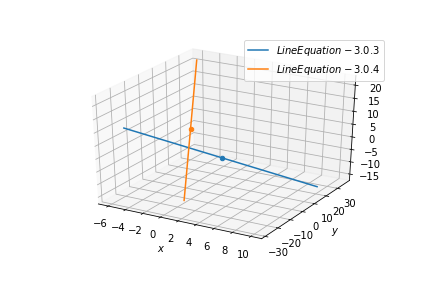
\includegraphics[width=\columnwidth]{./solutions/line_plane/74/codes/figs/Line_interest_1.png}
	\caption{Graph for equations \ref{eq:solutions/line_plane/74/codes7}}
	\label{fig:solutions/line_plane/74/codesline_equation_1}
\end{figure}


	\item 
	\begin{align}\label{eq:solutions/line_plane/74/codes12}
		\frac{x}{2} = \frac{y}{2} &= \frac{z}{1}, 
	\end{align}
	\begin{align}\label{eq:solutions/line_plane/74/codes13}
		\frac{x-5}{4} = \frac{y-2}{1} &= \frac{z-3}{8} 
	\end{align}



The above symmetric equations \ref{eq:solutions/line_plane/74/codes12}, \ref{eq:solutions/line_plane/74/codes13} can be represented in the vector form as 
\begin{align}\label{eq:solutions/line_plane/74/codes14}
	\quad \vec{r_1} &= \myvec{0\\0\\0} + \lambda_1\myvec{2\\2\\1}
	\\
	\quad \vec{r_2} &= \myvec{5\\2\\3} + \lambda_2\myvec{4\\1\\8}
\end{align}

As we have to find the angle between the vectors, we will only be taking the direction vectors into consideration. The direction vectors are $\vec{u}$ = $\myvec{2\\2\\1}$ and $\vec{v}$ = $\myvec{4\\1\\8}$. We can find the corresponding magnitude values

\begin{align}\label{eq:solutions/line_plane/74/codes16}
	\norm{\vec{u}} =\sqrt{2^{2}+2^{2}+1^{2}} =\sqrt{9}
\end{align}
\begin{align}\label{eq:solutions/line_plane/74/codes17}
	\norm{\vec{v}} =\sqrt{4^{2}+1^{2}+8^{2}} =\sqrt{81}
\end{align}

Using \ref{eq:solutions/line_plane/74/codes4}, \ref{eq:solutions/line_plane/74/codes16}, \ref{eq:solutions/line_plane/74/codes17} we get
\begin{align}
	\theta = \cos ^{-1}\frac{\myvec{2\\2\\1}^{T}\myvec{4\\1\\8}}{(\sqrt{9})(\sqrt{81})} 
	\\
	\theta = \cos ^{-1}\frac{18}{27.00}
	\\
	\theta = \cos ^{-1} (0.667)
	\\
	\theta = 48.189\degree
\end{align}

Therefore, the angle between the two lines is $48.189\degree$. See Fig. \ref{fig:solutions/line_plane/74/codesline_equation_2}


\begin{figure}
	\centering
	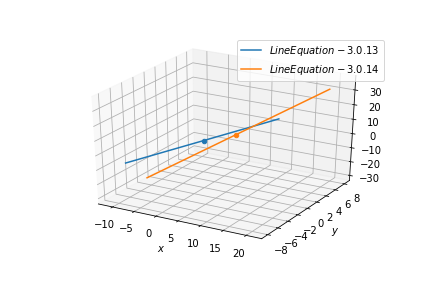
\includegraphics[width=\columnwidth]{./solutions/line_plane/74/codes/figs/Line_interest_2.png}
	\caption{Graph for equations \ref{eq:solutions/line_plane/74/codes14}}
	\label{fig:solutions/line_plane/74/codesline_equation_2}
\end{figure}
\end{enumerate}

    


\subsection{Complex Numbers}
\subsubsection{Problem}
Sketch the circles with
\begin{align}
\brak{a}centre \myvec{0\\2}, radius 2
\\
\brak{b}centre \myvec{-2\\32}, radius 4
\\
\brak{c}centre \myvec{\frac{1}{2}\\\frac{1}{4}}, radius \frac{1}{12}
\\
\brak{d}centre \myvec{1\\1}, radius \sqrt{2}
\\
\brak{e}centre \myvec{-a\\-b}, radius \sqrt{a^2-b^2}
\end{align}

\subsubsection{Solution}
\begin{align}
\myvec{1\\1} &= \sqrt{2}\myvec{\frac{1}{\sqrt{2}}\\ \frac{1}{\sqrt{2}}}
\\
&= \sqrt{2}\myvec{\cos 45\degree \\ \sin 45\degree}
\label{eq:3.4.7}
\end{align}
In the above, the modulus is $\norm{\myvec{1\\1}}=\sqrt{2}$ and the argument is $45 \degree$.
Similarly, 
\begin{align}
\myvec{1\\-1} &= \sqrt{2}\myvec{\cos 45\degree \\ -\sin 45\degree}
\\
\implies \myvec{1\\-1}^{-1} &= \frac{1}{\sqrt{2}}\myvec{\cos 45\degree \\ \sin 45\degree}
\end{align}
Using the matrix representation, 
\begin{align}
\frac{\myvec{1\\1}}{\myvec{1\\-1}} &= \myvec{\cos45\degree&-\sin45\degree\\\sin45\degree&\cos45\degree}
\nonumber \\
&\quad \times  \myvec{\cos45\degree&-\sin45\degree\\\sin45\degree&\cos45\degree}
\myvec{1\\0}
\\
 &= \myvec{\cos 90\degree\\ \sin 90\degree}= 1 \phase{90\degree}\end{align}
%
In general, if
\begin{align}
\vec{z}_1 &= r_1\myvec{\cos\theta_1\\\sin\theta_1}, \vec{z}_2 = r_2\myvec{\cos\theta_2\\\sin\theta_2},
\\
\vec{z}_1\vec{z}_2 &= r_1r_2\myvec{\cos(\theta_1+\theta_2)\\\sin(\theta_1+\theta_2)}.
\end{align}
Similarly, from \eqref{eq:3.4.7},
\begin{align}
\frac{1}{\myvec{1\\1}} &= \frac{1}{\sqrt{2}}\myvec{\cos 45\degree \\ -\sin 45\degree}
\\
&= \frac{1}{\sqrt{2}}\phase{-45\degree}
\end{align}


\subsection{Points and Vectors}
\subsubsection{Problem}
Sketch the circles with
\begin{align}
\brak{a}centre \myvec{0\\2}, radius 2
\\
\brak{b}centre \myvec{-2\\32}, radius 4
\\
\brak{c}centre \myvec{\frac{1}{2}\\\frac{1}{4}}, radius \frac{1}{12}
\\
\brak{d}centre \myvec{1\\1}, radius \sqrt{2}
\\
\brak{e}centre \myvec{-a\\-b}, radius \sqrt{a^2-b^2}
\end{align}

\subsubsection{Solution}
From theory, we understand that using dot product we can find the angle between the lines 
\begin{enumerate}
	\item 
	\begin{align}\label{eq:solutions/line_plane/74/codes:5}
		\frac{x-2}{2} = \frac{y-1}{5} &= \frac{z+3}{-3}, 
	\end{align}
	\begin{align}\label{eq:solutions/line_plane/74/codes:6}
		\frac{x+2}{-1} = \frac{y-4}{8} &= \frac{z-5}{4} 
	\end{align}


The above symmetric equations \ref{eq:solutions/line_plane/74/codes:5}, \ref{eq:solutions/line_plane/74/codes:6} can be represented in the vector form as 
\begin{align}\label{eq:solutions/line_plane/74/codes7}
	\quad \vec{r_1} &= \myvec{2\\1\\-3} + \lambda_1\myvec{2\\5\\-3}
	\\
	\quad \vec{r_2} &= \myvec{-2\\4\\5} + \lambda_2\myvec{-1\\8\\4}
\end{align}

As we have to find the angle between the vectors, we will only be taking the direction vectors into consideration. The direction vectors are $\vec{u}$ = $\myvec{2\\5\\-3}$ and $\vec{v}$ = $\myvec{-1\\8\\4}$. We can find the corresponding magnitude values

\begin{align}\label{eq:solutions/line_plane/74/codes9}
	\norm{\vec{u}} =\sqrt{2^{2}+5^{2}+(-3)^{2}} =\sqrt{38}
\end{align}
\begin{align}\label{eq:solutions/line_plane/74/codes10}
	\norm{\vec{v}} =\sqrt{(-1)^{2}+8^{2}+4^{2}} =\sqrt{81}
\end{align}

Using \ref{eq:solutions/line_plane/74/codes4}, \ref{eq:solutions/line_plane/74/codes9}, \ref{eq:solutions/line_plane/74/codes10} we get
\begin{align}
	\theta = \cos ^{-1}\frac{\myvec{2\\5\\-3}^{T}\myvec{-1\\8\\4}}{(\sqrt{38})(\sqrt{81})} 
	\\
	\theta = \cos ^{-1}\frac{26}{55.4797}
	\\
	\theta = \cos ^{-1} (0.4686)
	\\
	\theta = 62.053\degree
\end{align}

Therefore, the angle between the two lines is $62.053\degree$.See Fig. \ref{fig:solutions/line_plane/74/codesline_equation_1}

\begin{figure}
	\centering
	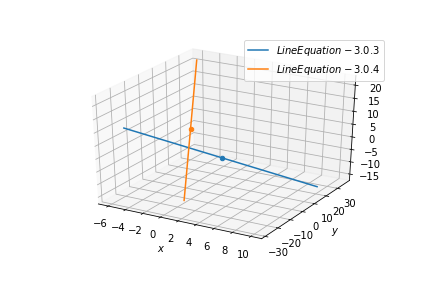
\includegraphics[width=\columnwidth]{./solutions/line_plane/74/codes/figs/Line_interest_1.png}
	\caption{Graph for equations \ref{eq:solutions/line_plane/74/codes7}}
	\label{fig:solutions/line_plane/74/codesline_equation_1}
\end{figure}


	\item 
	\begin{align}\label{eq:solutions/line_plane/74/codes12}
		\frac{x}{2} = \frac{y}{2} &= \frac{z}{1}, 
	\end{align}
	\begin{align}\label{eq:solutions/line_plane/74/codes13}
		\frac{x-5}{4} = \frac{y-2}{1} &= \frac{z-3}{8} 
	\end{align}



The above symmetric equations \ref{eq:solutions/line_plane/74/codes12}, \ref{eq:solutions/line_plane/74/codes13} can be represented in the vector form as 
\begin{align}\label{eq:solutions/line_plane/74/codes14}
	\quad \vec{r_1} &= \myvec{0\\0\\0} + \lambda_1\myvec{2\\2\\1}
	\\
	\quad \vec{r_2} &= \myvec{5\\2\\3} + \lambda_2\myvec{4\\1\\8}
\end{align}

As we have to find the angle between the vectors, we will only be taking the direction vectors into consideration. The direction vectors are $\vec{u}$ = $\myvec{2\\2\\1}$ and $\vec{v}$ = $\myvec{4\\1\\8}$. We can find the corresponding magnitude values

\begin{align}\label{eq:solutions/line_plane/74/codes16}
	\norm{\vec{u}} =\sqrt{2^{2}+2^{2}+1^{2}} =\sqrt{9}
\end{align}
\begin{align}\label{eq:solutions/line_plane/74/codes17}
	\norm{\vec{v}} =\sqrt{4^{2}+1^{2}+8^{2}} =\sqrt{81}
\end{align}

Using \ref{eq:solutions/line_plane/74/codes4}, \ref{eq:solutions/line_plane/74/codes16}, \ref{eq:solutions/line_plane/74/codes17} we get
\begin{align}
	\theta = \cos ^{-1}\frac{\myvec{2\\2\\1}^{T}\myvec{4\\1\\8}}{(\sqrt{9})(\sqrt{81})} 
	\\
	\theta = \cos ^{-1}\frac{18}{27.00}
	\\
	\theta = \cos ^{-1} (0.667)
	\\
	\theta = 48.189\degree
\end{align}

Therefore, the angle between the two lines is $48.189\degree$. See Fig. \ref{fig:solutions/line_plane/74/codesline_equation_2}


\begin{figure}
	\centering
	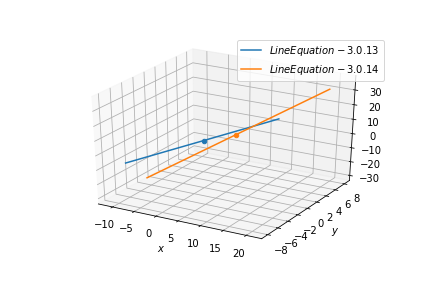
\includegraphics[width=\columnwidth]{./solutions/line_plane/74/codes/figs/Line_interest_2.png}
	\caption{Graph for equations \ref{eq:solutions/line_plane/74/codes14}}
	\label{fig:solutions/line_plane/74/codesline_equation_2}
\end{figure}
\end{enumerate}

    



\subsection{Points on a Line}
\subsubsection{Problem}
Sketch the circles with
\begin{align}
\brak{a}centre \myvec{0\\2}, radius 2
\\
\brak{b}centre \myvec{-2\\32}, radius 4
\\
\brak{c}centre \myvec{\frac{1}{2}\\\frac{1}{4}}, radius \frac{1}{12}
\\
\brak{d}centre \myvec{1\\1}, radius \sqrt{2}
\\
\brak{e}centre \myvec{-a\\-b}, radius \sqrt{a^2-b^2}
\end{align}

\subsubsection{Solution}
From theory, we understand that using dot product we can find the angle between the lines 
\begin{enumerate}
	\item 
	\begin{align}\label{eq:solutions/line_plane/74/codes:5}
		\frac{x-2}{2} = \frac{y-1}{5} &= \frac{z+3}{-3}, 
	\end{align}
	\begin{align}\label{eq:solutions/line_plane/74/codes:6}
		\frac{x+2}{-1} = \frac{y-4}{8} &= \frac{z-5}{4} 
	\end{align}


The above symmetric equations \ref{eq:solutions/line_plane/74/codes:5}, \ref{eq:solutions/line_plane/74/codes:6} can be represented in the vector form as 
\begin{align}\label{eq:solutions/line_plane/74/codes7}
	\quad \vec{r_1} &= \myvec{2\\1\\-3} + \lambda_1\myvec{2\\5\\-3}
	\\
	\quad \vec{r_2} &= \myvec{-2\\4\\5} + \lambda_2\myvec{-1\\8\\4}
\end{align}

As we have to find the angle between the vectors, we will only be taking the direction vectors into consideration. The direction vectors are $\vec{u}$ = $\myvec{2\\5\\-3}$ and $\vec{v}$ = $\myvec{-1\\8\\4}$. We can find the corresponding magnitude values

\begin{align}\label{eq:solutions/line_plane/74/codes9}
	\norm{\vec{u}} =\sqrt{2^{2}+5^{2}+(-3)^{2}} =\sqrt{38}
\end{align}
\begin{align}\label{eq:solutions/line_plane/74/codes10}
	\norm{\vec{v}} =\sqrt{(-1)^{2}+8^{2}+4^{2}} =\sqrt{81}
\end{align}

Using \ref{eq:solutions/line_plane/74/codes4}, \ref{eq:solutions/line_plane/74/codes9}, \ref{eq:solutions/line_plane/74/codes10} we get
\begin{align}
	\theta = \cos ^{-1}\frac{\myvec{2\\5\\-3}^{T}\myvec{-1\\8\\4}}{(\sqrt{38})(\sqrt{81})} 
	\\
	\theta = \cos ^{-1}\frac{26}{55.4797}
	\\
	\theta = \cos ^{-1} (0.4686)
	\\
	\theta = 62.053\degree
\end{align}

Therefore, the angle between the two lines is $62.053\degree$.See Fig. \ref{fig:solutions/line_plane/74/codesline_equation_1}

\begin{figure}
	\centering
	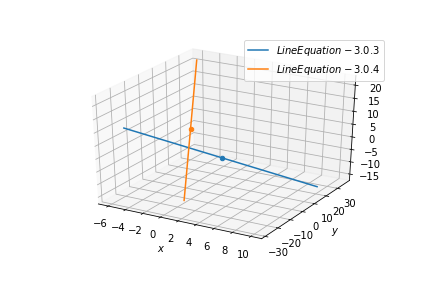
\includegraphics[width=\columnwidth]{./solutions/line_plane/74/codes/figs/Line_interest_1.png}
	\caption{Graph for equations \ref{eq:solutions/line_plane/74/codes7}}
	\label{fig:solutions/line_plane/74/codesline_equation_1}
\end{figure}


	\item 
	\begin{align}\label{eq:solutions/line_plane/74/codes12}
		\frac{x}{2} = \frac{y}{2} &= \frac{z}{1}, 
	\end{align}
	\begin{align}\label{eq:solutions/line_plane/74/codes13}
		\frac{x-5}{4} = \frac{y-2}{1} &= \frac{z-3}{8} 
	\end{align}



The above symmetric equations \ref{eq:solutions/line_plane/74/codes12}, \ref{eq:solutions/line_plane/74/codes13} can be represented in the vector form as 
\begin{align}\label{eq:solutions/line_plane/74/codes14}
	\quad \vec{r_1} &= \myvec{0\\0\\0} + \lambda_1\myvec{2\\2\\1}
	\\
	\quad \vec{r_2} &= \myvec{5\\2\\3} + \lambda_2\myvec{4\\1\\8}
\end{align}

As we have to find the angle between the vectors, we will only be taking the direction vectors into consideration. The direction vectors are $\vec{u}$ = $\myvec{2\\2\\1}$ and $\vec{v}$ = $\myvec{4\\1\\8}$. We can find the corresponding magnitude values

\begin{align}\label{eq:solutions/line_plane/74/codes16}
	\norm{\vec{u}} =\sqrt{2^{2}+2^{2}+1^{2}} =\sqrt{9}
\end{align}
\begin{align}\label{eq:solutions/line_plane/74/codes17}
	\norm{\vec{v}} =\sqrt{4^{2}+1^{2}+8^{2}} =\sqrt{81}
\end{align}

Using \ref{eq:solutions/line_plane/74/codes4}, \ref{eq:solutions/line_plane/74/codes16}, \ref{eq:solutions/line_plane/74/codes17} we get
\begin{align}
	\theta = \cos ^{-1}\frac{\myvec{2\\2\\1}^{T}\myvec{4\\1\\8}}{(\sqrt{9})(\sqrt{81})} 
	\\
	\theta = \cos ^{-1}\frac{18}{27.00}
	\\
	\theta = \cos ^{-1} (0.667)
	\\
	\theta = 48.189\degree
\end{align}

Therefore, the angle between the two lines is $48.189\degree$. See Fig. \ref{fig:solutions/line_plane/74/codesline_equation_2}


\begin{figure}
	\centering
	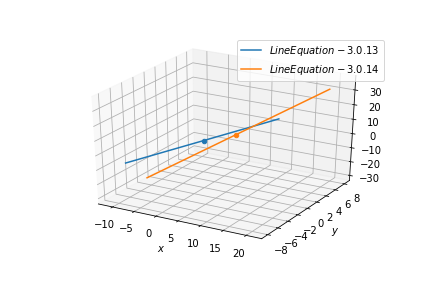
\includegraphics[width=\columnwidth]{./solutions/line_plane/74/codes/figs/Line_interest_2.png}
	\caption{Graph for equations \ref{eq:solutions/line_plane/74/codes14}}
	\label{fig:solutions/line_plane/74/codesline_equation_2}
\end{figure}
\end{enumerate}

    


\subsection{Lines and Plane }
\subsubsection{Problem}
Sketch the circles with
\begin{align}
\brak{a}centre \myvec{0\\2}, radius 2
\\
\brak{b}centre \myvec{-2\\32}, radius 4
\\
\brak{c}centre \myvec{\frac{1}{2}\\\frac{1}{4}}, radius \frac{1}{12}
\\
\brak{d}centre \myvec{1\\1}, radius \sqrt{2}
\\
\brak{e}centre \myvec{-a\\-b}, radius \sqrt{a^2-b^2}
\end{align}

\subsubsection{Solution}
From theory, we understand that using dot product we can find the angle between the lines 
\begin{enumerate}
	\item 
	\begin{align}\label{eq:solutions/line_plane/74/codes:5}
		\frac{x-2}{2} = \frac{y-1}{5} &= \frac{z+3}{-3}, 
	\end{align}
	\begin{align}\label{eq:solutions/line_plane/74/codes:6}
		\frac{x+2}{-1} = \frac{y-4}{8} &= \frac{z-5}{4} 
	\end{align}


The above symmetric equations \ref{eq:solutions/line_plane/74/codes:5}, \ref{eq:solutions/line_plane/74/codes:6} can be represented in the vector form as 
\begin{align}\label{eq:solutions/line_plane/74/codes7}
	\quad \vec{r_1} &= \myvec{2\\1\\-3} + \lambda_1\myvec{2\\5\\-3}
	\\
	\quad \vec{r_2} &= \myvec{-2\\4\\5} + \lambda_2\myvec{-1\\8\\4}
\end{align}

As we have to find the angle between the vectors, we will only be taking the direction vectors into consideration. The direction vectors are $\vec{u}$ = $\myvec{2\\5\\-3}$ and $\vec{v}$ = $\myvec{-1\\8\\4}$. We can find the corresponding magnitude values

\begin{align}\label{eq:solutions/line_plane/74/codes9}
	\norm{\vec{u}} =\sqrt{2^{2}+5^{2}+(-3)^{2}} =\sqrt{38}
\end{align}
\begin{align}\label{eq:solutions/line_plane/74/codes10}
	\norm{\vec{v}} =\sqrt{(-1)^{2}+8^{2}+4^{2}} =\sqrt{81}
\end{align}

Using \ref{eq:solutions/line_plane/74/codes4}, \ref{eq:solutions/line_plane/74/codes9}, \ref{eq:solutions/line_plane/74/codes10} we get
\begin{align}
	\theta = \cos ^{-1}\frac{\myvec{2\\5\\-3}^{T}\myvec{-1\\8\\4}}{(\sqrt{38})(\sqrt{81})} 
	\\
	\theta = \cos ^{-1}\frac{26}{55.4797}
	\\
	\theta = \cos ^{-1} (0.4686)
	\\
	\theta = 62.053\degree
\end{align}

Therefore, the angle between the two lines is $62.053\degree$.See Fig. \ref{fig:solutions/line_plane/74/codesline_equation_1}

\begin{figure}
	\centering
	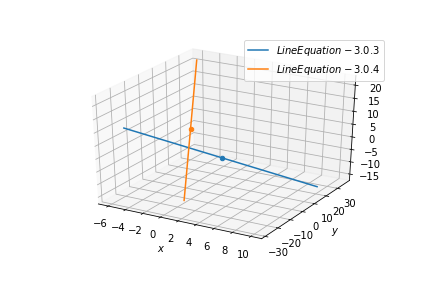
\includegraphics[width=\columnwidth]{./solutions/line_plane/74/codes/figs/Line_interest_1.png}
	\caption{Graph for equations \ref{eq:solutions/line_plane/74/codes7}}
	\label{fig:solutions/line_plane/74/codesline_equation_1}
\end{figure}


	\item 
	\begin{align}\label{eq:solutions/line_plane/74/codes12}
		\frac{x}{2} = \frac{y}{2} &= \frac{z}{1}, 
	\end{align}
	\begin{align}\label{eq:solutions/line_plane/74/codes13}
		\frac{x-5}{4} = \frac{y-2}{1} &= \frac{z-3}{8} 
	\end{align}



The above symmetric equations \ref{eq:solutions/line_plane/74/codes12}, \ref{eq:solutions/line_plane/74/codes13} can be represented in the vector form as 
\begin{align}\label{eq:solutions/line_plane/74/codes14}
	\quad \vec{r_1} &= \myvec{0\\0\\0} + \lambda_1\myvec{2\\2\\1}
	\\
	\quad \vec{r_2} &= \myvec{5\\2\\3} + \lambda_2\myvec{4\\1\\8}
\end{align}

As we have to find the angle between the vectors, we will only be taking the direction vectors into consideration. The direction vectors are $\vec{u}$ = $\myvec{2\\2\\1}$ and $\vec{v}$ = $\myvec{4\\1\\8}$. We can find the corresponding magnitude values

\begin{align}\label{eq:solutions/line_plane/74/codes16}
	\norm{\vec{u}} =\sqrt{2^{2}+2^{2}+1^{2}} =\sqrt{9}
\end{align}
\begin{align}\label{eq:solutions/line_plane/74/codes17}
	\norm{\vec{v}} =\sqrt{4^{2}+1^{2}+8^{2}} =\sqrt{81}
\end{align}

Using \ref{eq:solutions/line_plane/74/codes4}, \ref{eq:solutions/line_plane/74/codes16}, \ref{eq:solutions/line_plane/74/codes17} we get
\begin{align}
	\theta = \cos ^{-1}\frac{\myvec{2\\2\\1}^{T}\myvec{4\\1\\8}}{(\sqrt{9})(\sqrt{81})} 
	\\
	\theta = \cos ^{-1}\frac{18}{27.00}
	\\
	\theta = \cos ^{-1} (0.667)
	\\
	\theta = 48.189\degree
\end{align}

Therefore, the angle between the two lines is $48.189\degree$. See Fig. \ref{fig:solutions/line_plane/74/codesline_equation_2}


\begin{figure}
	\centering
	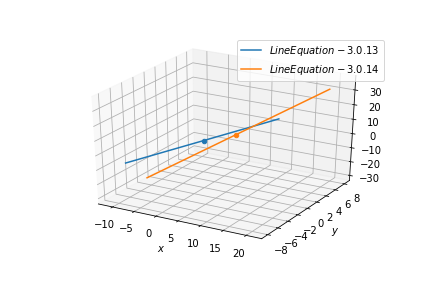
\includegraphics[width=\columnwidth]{./solutions/line_plane/74/codes/figs/Line_interest_2.png}
	\caption{Graph for equations \ref{eq:solutions/line_plane/74/codes14}}
	\label{fig:solutions/line_plane/74/codesline_equation_2}
\end{figure}
\end{enumerate}

    


\subsection{Motion in a Plane}
\subsubsection{Problem}
Sketch the circles with
\begin{align}
\brak{a}centre \myvec{0\\2}, radius 2
\\
\brak{b}centre \myvec{-2\\32}, radius 4
\\
\brak{c}centre \myvec{\frac{1}{2}\\\frac{1}{4}}, radius \frac{1}{12}
\\
\brak{d}centre \myvec{1\\1}, radius \sqrt{2}
\\
\brak{e}centre \myvec{-a\\-b}, radius \sqrt{a^2-b^2}
\end{align}

\subsubsection{Solution}
From theory, we understand that using dot product we can find the angle between the lines 
\begin{enumerate}
	\item 
	\begin{align}\label{eq:solutions/line_plane/74/codes:5}
		\frac{x-2}{2} = \frac{y-1}{5} &= \frac{z+3}{-3}, 
	\end{align}
	\begin{align}\label{eq:solutions/line_plane/74/codes:6}
		\frac{x+2}{-1} = \frac{y-4}{8} &= \frac{z-5}{4} 
	\end{align}


The above symmetric equations \ref{eq:solutions/line_plane/74/codes:5}, \ref{eq:solutions/line_plane/74/codes:6} can be represented in the vector form as 
\begin{align}\label{eq:solutions/line_plane/74/codes7}
	\quad \vec{r_1} &= \myvec{2\\1\\-3} + \lambda_1\myvec{2\\5\\-3}
	\\
	\quad \vec{r_2} &= \myvec{-2\\4\\5} + \lambda_2\myvec{-1\\8\\4}
\end{align}

As we have to find the angle between the vectors, we will only be taking the direction vectors into consideration. The direction vectors are $\vec{u}$ = $\myvec{2\\5\\-3}$ and $\vec{v}$ = $\myvec{-1\\8\\4}$. We can find the corresponding magnitude values

\begin{align}\label{eq:solutions/line_plane/74/codes9}
	\norm{\vec{u}} =\sqrt{2^{2}+5^{2}+(-3)^{2}} =\sqrt{38}
\end{align}
\begin{align}\label{eq:solutions/line_plane/74/codes10}
	\norm{\vec{v}} =\sqrt{(-1)^{2}+8^{2}+4^{2}} =\sqrt{81}
\end{align}

Using \ref{eq:solutions/line_plane/74/codes4}, \ref{eq:solutions/line_plane/74/codes9}, \ref{eq:solutions/line_plane/74/codes10} we get
\begin{align}
	\theta = \cos ^{-1}\frac{\myvec{2\\5\\-3}^{T}\myvec{-1\\8\\4}}{(\sqrt{38})(\sqrt{81})} 
	\\
	\theta = \cos ^{-1}\frac{26}{55.4797}
	\\
	\theta = \cos ^{-1} (0.4686)
	\\
	\theta = 62.053\degree
\end{align}

Therefore, the angle between the two lines is $62.053\degree$.See Fig. \ref{fig:solutions/line_plane/74/codesline_equation_1}

\begin{figure}
	\centering
	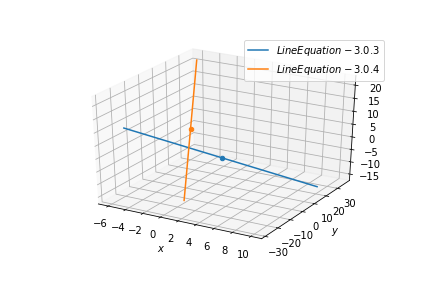
\includegraphics[width=\columnwidth]{./solutions/line_plane/74/codes/figs/Line_interest_1.png}
	\caption{Graph for equations \ref{eq:solutions/line_plane/74/codes7}}
	\label{fig:solutions/line_plane/74/codesline_equation_1}
\end{figure}


	\item 
	\begin{align}\label{eq:solutions/line_plane/74/codes12}
		\frac{x}{2} = \frac{y}{2} &= \frac{z}{1}, 
	\end{align}
	\begin{align}\label{eq:solutions/line_plane/74/codes13}
		\frac{x-5}{4} = \frac{y-2}{1} &= \frac{z-3}{8} 
	\end{align}



The above symmetric equations \ref{eq:solutions/line_plane/74/codes12}, \ref{eq:solutions/line_plane/74/codes13} can be represented in the vector form as 
\begin{align}\label{eq:solutions/line_plane/74/codes14}
	\quad \vec{r_1} &= \myvec{0\\0\\0} + \lambda_1\myvec{2\\2\\1}
	\\
	\quad \vec{r_2} &= \myvec{5\\2\\3} + \lambda_2\myvec{4\\1\\8}
\end{align}

As we have to find the angle between the vectors, we will only be taking the direction vectors into consideration. The direction vectors are $\vec{u}$ = $\myvec{2\\2\\1}$ and $\vec{v}$ = $\myvec{4\\1\\8}$. We can find the corresponding magnitude values

\begin{align}\label{eq:solutions/line_plane/74/codes16}
	\norm{\vec{u}} =\sqrt{2^{2}+2^{2}+1^{2}} =\sqrt{9}
\end{align}
\begin{align}\label{eq:solutions/line_plane/74/codes17}
	\norm{\vec{v}} =\sqrt{4^{2}+1^{2}+8^{2}} =\sqrt{81}
\end{align}

Using \ref{eq:solutions/line_plane/74/codes4}, \ref{eq:solutions/line_plane/74/codes16}, \ref{eq:solutions/line_plane/74/codes17} we get
\begin{align}
	\theta = \cos ^{-1}\frac{\myvec{2\\2\\1}^{T}\myvec{4\\1\\8}}{(\sqrt{9})(\sqrt{81})} 
	\\
	\theta = \cos ^{-1}\frac{18}{27.00}
	\\
	\theta = \cos ^{-1} (0.667)
	\\
	\theta = 48.189\degree
\end{align}

Therefore, the angle between the two lines is $48.189\degree$. See Fig. \ref{fig:solutions/line_plane/74/codesline_equation_2}


\begin{figure}
	\centering
	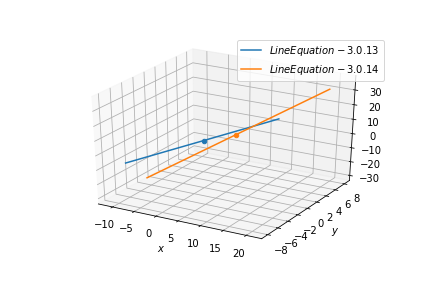
\includegraphics[width=\columnwidth]{./solutions/line_plane/74/codes/figs/Line_interest_2.png}
	\caption{Graph for equations \ref{eq:solutions/line_plane/74/codes14}}
	\label{fig:solutions/line_plane/74/codesline_equation_2}
\end{figure}
\end{enumerate}

    


\subsection{Determinants}
\subsubsection{Problem}
Sketch the circles with
\begin{align}
\brak{a}centre \myvec{0\\2}, radius 2
\\
\brak{b}centre \myvec{-2\\32}, radius 4
\\
\brak{c}centre \myvec{\frac{1}{2}\\\frac{1}{4}}, radius \frac{1}{12}
\\
\brak{d}centre \myvec{1\\1}, radius \sqrt{2}
\\
\brak{e}centre \myvec{-a\\-b}, radius \sqrt{a^2-b^2}
\end{align}

\subsubsection{Solution}
From theory, we understand that using dot product we can find the angle between the lines 
\begin{enumerate}
	\item 
	\begin{align}\label{eq:solutions/line_plane/74/codes:5}
		\frac{x-2}{2} = \frac{y-1}{5} &= \frac{z+3}{-3}, 
	\end{align}
	\begin{align}\label{eq:solutions/line_plane/74/codes:6}
		\frac{x+2}{-1} = \frac{y-4}{8} &= \frac{z-5}{4} 
	\end{align}


The above symmetric equations \ref{eq:solutions/line_plane/74/codes:5}, \ref{eq:solutions/line_plane/74/codes:6} can be represented in the vector form as 
\begin{align}\label{eq:solutions/line_plane/74/codes7}
	\quad \vec{r_1} &= \myvec{2\\1\\-3} + \lambda_1\myvec{2\\5\\-3}
	\\
	\quad \vec{r_2} &= \myvec{-2\\4\\5} + \lambda_2\myvec{-1\\8\\4}
\end{align}

As we have to find the angle between the vectors, we will only be taking the direction vectors into consideration. The direction vectors are $\vec{u}$ = $\myvec{2\\5\\-3}$ and $\vec{v}$ = $\myvec{-1\\8\\4}$. We can find the corresponding magnitude values

\begin{align}\label{eq:solutions/line_plane/74/codes9}
	\norm{\vec{u}} =\sqrt{2^{2}+5^{2}+(-3)^{2}} =\sqrt{38}
\end{align}
\begin{align}\label{eq:solutions/line_plane/74/codes10}
	\norm{\vec{v}} =\sqrt{(-1)^{2}+8^{2}+4^{2}} =\sqrt{81}
\end{align}

Using \ref{eq:solutions/line_plane/74/codes4}, \ref{eq:solutions/line_plane/74/codes9}, \ref{eq:solutions/line_plane/74/codes10} we get
\begin{align}
	\theta = \cos ^{-1}\frac{\myvec{2\\5\\-3}^{T}\myvec{-1\\8\\4}}{(\sqrt{38})(\sqrt{81})} 
	\\
	\theta = \cos ^{-1}\frac{26}{55.4797}
	\\
	\theta = \cos ^{-1} (0.4686)
	\\
	\theta = 62.053\degree
\end{align}

Therefore, the angle between the two lines is $62.053\degree$.See Fig. \ref{fig:solutions/line_plane/74/codesline_equation_1}

\begin{figure}
	\centering
	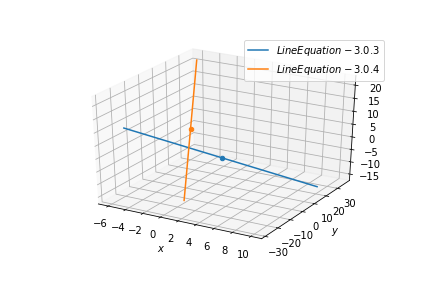
\includegraphics[width=\columnwidth]{./solutions/line_plane/74/codes/figs/Line_interest_1.png}
	\caption{Graph for equations \ref{eq:solutions/line_plane/74/codes7}}
	\label{fig:solutions/line_plane/74/codesline_equation_1}
\end{figure}


	\item 
	\begin{align}\label{eq:solutions/line_plane/74/codes12}
		\frac{x}{2} = \frac{y}{2} &= \frac{z}{1}, 
	\end{align}
	\begin{align}\label{eq:solutions/line_plane/74/codes13}
		\frac{x-5}{4} = \frac{y-2}{1} &= \frac{z-3}{8} 
	\end{align}



The above symmetric equations \ref{eq:solutions/line_plane/74/codes12}, \ref{eq:solutions/line_plane/74/codes13} can be represented in the vector form as 
\begin{align}\label{eq:solutions/line_plane/74/codes14}
	\quad \vec{r_1} &= \myvec{0\\0\\0} + \lambda_1\myvec{2\\2\\1}
	\\
	\quad \vec{r_2} &= \myvec{5\\2\\3} + \lambda_2\myvec{4\\1\\8}
\end{align}

As we have to find the angle between the vectors, we will only be taking the direction vectors into consideration. The direction vectors are $\vec{u}$ = $\myvec{2\\2\\1}$ and $\vec{v}$ = $\myvec{4\\1\\8}$. We can find the corresponding magnitude values

\begin{align}\label{eq:solutions/line_plane/74/codes16}
	\norm{\vec{u}} =\sqrt{2^{2}+2^{2}+1^{2}} =\sqrt{9}
\end{align}
\begin{align}\label{eq:solutions/line_plane/74/codes17}
	\norm{\vec{v}} =\sqrt{4^{2}+1^{2}+8^{2}} =\sqrt{81}
\end{align}

Using \ref{eq:solutions/line_plane/74/codes4}, \ref{eq:solutions/line_plane/74/codes16}, \ref{eq:solutions/line_plane/74/codes17} we get
\begin{align}
	\theta = \cos ^{-1}\frac{\myvec{2\\2\\1}^{T}\myvec{4\\1\\8}}{(\sqrt{9})(\sqrt{81})} 
	\\
	\theta = \cos ^{-1}\frac{18}{27.00}
	\\
	\theta = \cos ^{-1} (0.667)
	\\
	\theta = 48.189\degree
\end{align}

Therefore, the angle between the two lines is $48.189\degree$. See Fig. \ref{fig:solutions/line_plane/74/codesline_equation_2}


\begin{figure}
	\centering
	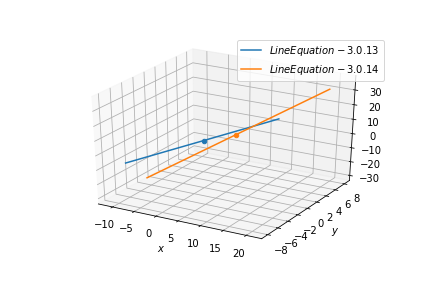
\includegraphics[width=\columnwidth]{./solutions/line_plane/74/codes/figs/Line_interest_2.png}
	\caption{Graph for equations \ref{eq:solutions/line_plane/74/codes14}}
	\label{fig:solutions/line_plane/74/codesline_equation_2}
\end{figure}
\end{enumerate}

    


\subsection{Linear Inequalities}
\subsubsection{Problem}
Sketch the circles with
\begin{align}
\brak{a}centre \myvec{0\\2}, radius 2
\\
\brak{b}centre \myvec{-2\\32}, radius 4
\\
\brak{c}centre \myvec{\frac{1}{2}\\\frac{1}{4}}, radius \frac{1}{12}
\\
\brak{d}centre \myvec{1\\1}, radius \sqrt{2}
\\
\brak{e}centre \myvec{-a\\-b}, radius \sqrt{a^2-b^2}
\end{align}

\subsubsection{Solution}
From theory, we understand that using dot product we can find the angle between the lines 
\begin{enumerate}
	\item 
	\begin{align}\label{eq:solutions/line_plane/74/codes:5}
		\frac{x-2}{2} = \frac{y-1}{5} &= \frac{z+3}{-3}, 
	\end{align}
	\begin{align}\label{eq:solutions/line_plane/74/codes:6}
		\frac{x+2}{-1} = \frac{y-4}{8} &= \frac{z-5}{4} 
	\end{align}


The above symmetric equations \ref{eq:solutions/line_plane/74/codes:5}, \ref{eq:solutions/line_plane/74/codes:6} can be represented in the vector form as 
\begin{align}\label{eq:solutions/line_plane/74/codes7}
	\quad \vec{r_1} &= \myvec{2\\1\\-3} + \lambda_1\myvec{2\\5\\-3}
	\\
	\quad \vec{r_2} &= \myvec{-2\\4\\5} + \lambda_2\myvec{-1\\8\\4}
\end{align}

As we have to find the angle between the vectors, we will only be taking the direction vectors into consideration. The direction vectors are $\vec{u}$ = $\myvec{2\\5\\-3}$ and $\vec{v}$ = $\myvec{-1\\8\\4}$. We can find the corresponding magnitude values

\begin{align}\label{eq:solutions/line_plane/74/codes9}
	\norm{\vec{u}} =\sqrt{2^{2}+5^{2}+(-3)^{2}} =\sqrt{38}
\end{align}
\begin{align}\label{eq:solutions/line_plane/74/codes10}
	\norm{\vec{v}} =\sqrt{(-1)^{2}+8^{2}+4^{2}} =\sqrt{81}
\end{align}

Using \ref{eq:solutions/line_plane/74/codes4}, \ref{eq:solutions/line_plane/74/codes9}, \ref{eq:solutions/line_plane/74/codes10} we get
\begin{align}
	\theta = \cos ^{-1}\frac{\myvec{2\\5\\-3}^{T}\myvec{-1\\8\\4}}{(\sqrt{38})(\sqrt{81})} 
	\\
	\theta = \cos ^{-1}\frac{26}{55.4797}
	\\
	\theta = \cos ^{-1} (0.4686)
	\\
	\theta = 62.053\degree
\end{align}

Therefore, the angle between the two lines is $62.053\degree$.See Fig. \ref{fig:solutions/line_plane/74/codesline_equation_1}

\begin{figure}
	\centering
	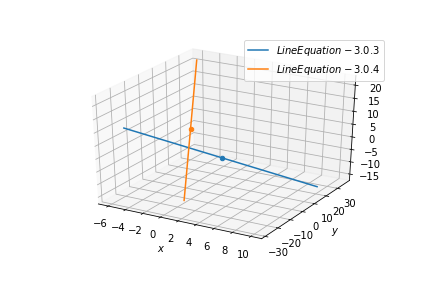
\includegraphics[width=\columnwidth]{./solutions/line_plane/74/codes/figs/Line_interest_1.png}
	\caption{Graph for equations \ref{eq:solutions/line_plane/74/codes7}}
	\label{fig:solutions/line_plane/74/codesline_equation_1}
\end{figure}


	\item 
	\begin{align}\label{eq:solutions/line_plane/74/codes12}
		\frac{x}{2} = \frac{y}{2} &= \frac{z}{1}, 
	\end{align}
	\begin{align}\label{eq:solutions/line_plane/74/codes13}
		\frac{x-5}{4} = \frac{y-2}{1} &= \frac{z-3}{8} 
	\end{align}



The above symmetric equations \ref{eq:solutions/line_plane/74/codes12}, \ref{eq:solutions/line_plane/74/codes13} can be represented in the vector form as 
\begin{align}\label{eq:solutions/line_plane/74/codes14}
	\quad \vec{r_1} &= \myvec{0\\0\\0} + \lambda_1\myvec{2\\2\\1}
	\\
	\quad \vec{r_2} &= \myvec{5\\2\\3} + \lambda_2\myvec{4\\1\\8}
\end{align}

As we have to find the angle between the vectors, we will only be taking the direction vectors into consideration. The direction vectors are $\vec{u}$ = $\myvec{2\\2\\1}$ and $\vec{v}$ = $\myvec{4\\1\\8}$. We can find the corresponding magnitude values

\begin{align}\label{eq:solutions/line_plane/74/codes16}
	\norm{\vec{u}} =\sqrt{2^{2}+2^{2}+1^{2}} =\sqrt{9}
\end{align}
\begin{align}\label{eq:solutions/line_plane/74/codes17}
	\norm{\vec{v}} =\sqrt{4^{2}+1^{2}+8^{2}} =\sqrt{81}
\end{align}

Using \ref{eq:solutions/line_plane/74/codes4}, \ref{eq:solutions/line_plane/74/codes16}, \ref{eq:solutions/line_plane/74/codes17} we get
\begin{align}
	\theta = \cos ^{-1}\frac{\myvec{2\\2\\1}^{T}\myvec{4\\1\\8}}{(\sqrt{9})(\sqrt{81})} 
	\\
	\theta = \cos ^{-1}\frac{18}{27.00}
	\\
	\theta = \cos ^{-1} (0.667)
	\\
	\theta = 48.189\degree
\end{align}

Therefore, the angle between the two lines is $48.189\degree$. See Fig. \ref{fig:solutions/line_plane/74/codesline_equation_2}


\begin{figure}
	\centering
	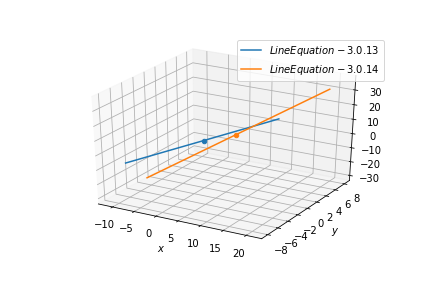
\includegraphics[width=\columnwidth]{./solutions/line_plane/74/codes/figs/Line_interest_2.png}
	\caption{Graph for equations \ref{eq:solutions/line_plane/74/codes14}}
	\label{fig:solutions/line_plane/74/codesline_equation_2}
\end{figure}
\end{enumerate}

    


\subsection{Miscellaneous}
\subsubsection{Problem}
Sketch the circles with
\begin{align}
\brak{a}centre \myvec{0\\2}, radius 2
\\
\brak{b}centre \myvec{-2\\32}, radius 4
\\
\brak{c}centre \myvec{\frac{1}{2}\\\frac{1}{4}}, radius \frac{1}{12}
\\
\brak{d}centre \myvec{1\\1}, radius \sqrt{2}
\\
\brak{e}centre \myvec{-a\\-b}, radius \sqrt{a^2-b^2}
\end{align}

\subsubsection{Solution}
From theory, we understand that using dot product we can find the angle between the lines 
\begin{enumerate}
	\item 
	\begin{align}\label{eq:solutions/line_plane/74/codes:5}
		\frac{x-2}{2} = \frac{y-1}{5} &= \frac{z+3}{-3}, 
	\end{align}
	\begin{align}\label{eq:solutions/line_plane/74/codes:6}
		\frac{x+2}{-1} = \frac{y-4}{8} &= \frac{z-5}{4} 
	\end{align}


The above symmetric equations \ref{eq:solutions/line_plane/74/codes:5}, \ref{eq:solutions/line_plane/74/codes:6} can be represented in the vector form as 
\begin{align}\label{eq:solutions/line_plane/74/codes7}
	\quad \vec{r_1} &= \myvec{2\\1\\-3} + \lambda_1\myvec{2\\5\\-3}
	\\
	\quad \vec{r_2} &= \myvec{-2\\4\\5} + \lambda_2\myvec{-1\\8\\4}
\end{align}

As we have to find the angle between the vectors, we will only be taking the direction vectors into consideration. The direction vectors are $\vec{u}$ = $\myvec{2\\5\\-3}$ and $\vec{v}$ = $\myvec{-1\\8\\4}$. We can find the corresponding magnitude values

\begin{align}\label{eq:solutions/line_plane/74/codes9}
	\norm{\vec{u}} =\sqrt{2^{2}+5^{2}+(-3)^{2}} =\sqrt{38}
\end{align}
\begin{align}\label{eq:solutions/line_plane/74/codes10}
	\norm{\vec{v}} =\sqrt{(-1)^{2}+8^{2}+4^{2}} =\sqrt{81}
\end{align}

Using \ref{eq:solutions/line_plane/74/codes4}, \ref{eq:solutions/line_plane/74/codes9}, \ref{eq:solutions/line_plane/74/codes10} we get
\begin{align}
	\theta = \cos ^{-1}\frac{\myvec{2\\5\\-3}^{T}\myvec{-1\\8\\4}}{(\sqrt{38})(\sqrt{81})} 
	\\
	\theta = \cos ^{-1}\frac{26}{55.4797}
	\\
	\theta = \cos ^{-1} (0.4686)
	\\
	\theta = 62.053\degree
\end{align}

Therefore, the angle between the two lines is $62.053\degree$.See Fig. \ref{fig:solutions/line_plane/74/codesline_equation_1}

\begin{figure}
	\centering
	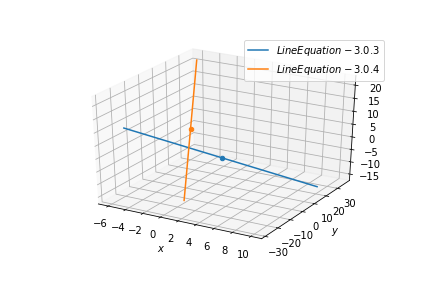
\includegraphics[width=\columnwidth]{./solutions/line_plane/74/codes/figs/Line_interest_1.png}
	\caption{Graph for equations \ref{eq:solutions/line_plane/74/codes7}}
	\label{fig:solutions/line_plane/74/codesline_equation_1}
\end{figure}


	\item 
	\begin{align}\label{eq:solutions/line_plane/74/codes12}
		\frac{x}{2} = \frac{y}{2} &= \frac{z}{1}, 
	\end{align}
	\begin{align}\label{eq:solutions/line_plane/74/codes13}
		\frac{x-5}{4} = \frac{y-2}{1} &= \frac{z-3}{8} 
	\end{align}



The above symmetric equations \ref{eq:solutions/line_plane/74/codes12}, \ref{eq:solutions/line_plane/74/codes13} can be represented in the vector form as 
\begin{align}\label{eq:solutions/line_plane/74/codes14}
	\quad \vec{r_1} &= \myvec{0\\0\\0} + \lambda_1\myvec{2\\2\\1}
	\\
	\quad \vec{r_2} &= \myvec{5\\2\\3} + \lambda_2\myvec{4\\1\\8}
\end{align}

As we have to find the angle between the vectors, we will only be taking the direction vectors into consideration. The direction vectors are $\vec{u}$ = $\myvec{2\\2\\1}$ and $\vec{v}$ = $\myvec{4\\1\\8}$. We can find the corresponding magnitude values

\begin{align}\label{eq:solutions/line_plane/74/codes16}
	\norm{\vec{u}} =\sqrt{2^{2}+2^{2}+1^{2}} =\sqrt{9}
\end{align}
\begin{align}\label{eq:solutions/line_plane/74/codes17}
	\norm{\vec{v}} =\sqrt{4^{2}+1^{2}+8^{2}} =\sqrt{81}
\end{align}

Using \ref{eq:solutions/line_plane/74/codes4}, \ref{eq:solutions/line_plane/74/codes16}, \ref{eq:solutions/line_plane/74/codes17} we get
\begin{align}
	\theta = \cos ^{-1}\frac{\myvec{2\\2\\1}^{T}\myvec{4\\1\\8}}{(\sqrt{9})(\sqrt{81})} 
	\\
	\theta = \cos ^{-1}\frac{18}{27.00}
	\\
	\theta = \cos ^{-1} (0.667)
	\\
	\theta = 48.189\degree
\end{align}

Therefore, the angle between the two lines is $48.189\degree$. See Fig. \ref{fig:solutions/line_plane/74/codesline_equation_2}


\begin{figure}
	\centering
	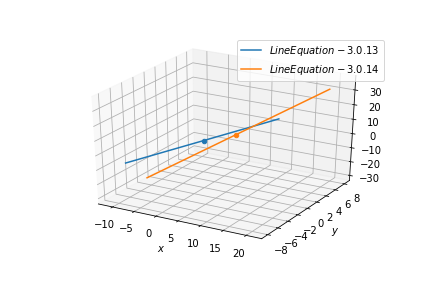
\includegraphics[width=\columnwidth]{./solutions/line_plane/74/codes/figs/Line_interest_2.png}
	\caption{Graph for equations \ref{eq:solutions/line_plane/74/codes14}}
	\label{fig:solutions/line_plane/74/codesline_equation_2}
\end{figure}
\end{enumerate}

    


\section{CIRCLE EXERCISE}
\subsection{Problem}
Sketch the circles with
\begin{align}
\brak{a}centre \myvec{0\\2}, radius 2
\\
\brak{b}centre \myvec{-2\\32}, radius 4
\\
\brak{c}centre \myvec{\frac{1}{2}\\\frac{1}{4}}, radius \frac{1}{12}
\\
\brak{d}centre \myvec{1\\1}, radius \sqrt{2}
\\
\brak{e}centre \myvec{-a\\-b}, radius \sqrt{a^2-b^2}
\end{align}

\subsection{Solution}
From theory, we understand that using dot product we can find the angle between the lines 
\begin{enumerate}
	\item 
	\begin{align}\label{eq:solutions/line_plane/74/codes:5}
		\frac{x-2}{2} = \frac{y-1}{5} &= \frac{z+3}{-3}, 
	\end{align}
	\begin{align}\label{eq:solutions/line_plane/74/codes:6}
		\frac{x+2}{-1} = \frac{y-4}{8} &= \frac{z-5}{4} 
	\end{align}


The above symmetric equations \ref{eq:solutions/line_plane/74/codes:5}, \ref{eq:solutions/line_plane/74/codes:6} can be represented in the vector form as 
\begin{align}\label{eq:solutions/line_plane/74/codes7}
	\quad \vec{r_1} &= \myvec{2\\1\\-3} + \lambda_1\myvec{2\\5\\-3}
	\\
	\quad \vec{r_2} &= \myvec{-2\\4\\5} + \lambda_2\myvec{-1\\8\\4}
\end{align}

As we have to find the angle between the vectors, we will only be taking the direction vectors into consideration. The direction vectors are $\vec{u}$ = $\myvec{2\\5\\-3}$ and $\vec{v}$ = $\myvec{-1\\8\\4}$. We can find the corresponding magnitude values

\begin{align}\label{eq:solutions/line_plane/74/codes9}
	\norm{\vec{u}} =\sqrt{2^{2}+5^{2}+(-3)^{2}} =\sqrt{38}
\end{align}
\begin{align}\label{eq:solutions/line_plane/74/codes10}
	\norm{\vec{v}} =\sqrt{(-1)^{2}+8^{2}+4^{2}} =\sqrt{81}
\end{align}

Using \ref{eq:solutions/line_plane/74/codes4}, \ref{eq:solutions/line_plane/74/codes9}, \ref{eq:solutions/line_plane/74/codes10} we get
\begin{align}
	\theta = \cos ^{-1}\frac{\myvec{2\\5\\-3}^{T}\myvec{-1\\8\\4}}{(\sqrt{38})(\sqrt{81})} 
	\\
	\theta = \cos ^{-1}\frac{26}{55.4797}
	\\
	\theta = \cos ^{-1} (0.4686)
	\\
	\theta = 62.053\degree
\end{align}

Therefore, the angle between the two lines is $62.053\degree$.See Fig. \ref{fig:solutions/line_plane/74/codesline_equation_1}

\begin{figure}
	\centering
	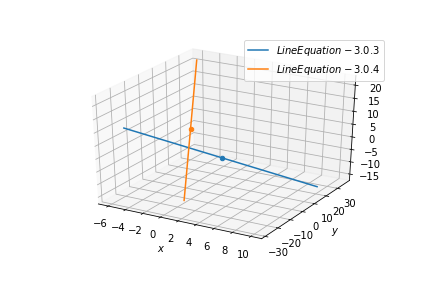
\includegraphics[width=\columnwidth]{./solutions/line_plane/74/codes/figs/Line_interest_1.png}
	\caption{Graph for equations \ref{eq:solutions/line_plane/74/codes7}}
	\label{fig:solutions/line_plane/74/codesline_equation_1}
\end{figure}


	\item 
	\begin{align}\label{eq:solutions/line_plane/74/codes12}
		\frac{x}{2} = \frac{y}{2} &= \frac{z}{1}, 
	\end{align}
	\begin{align}\label{eq:solutions/line_plane/74/codes13}
		\frac{x-5}{4} = \frac{y-2}{1} &= \frac{z-3}{8} 
	\end{align}



The above symmetric equations \ref{eq:solutions/line_plane/74/codes12}, \ref{eq:solutions/line_plane/74/codes13} can be represented in the vector form as 
\begin{align}\label{eq:solutions/line_plane/74/codes14}
	\quad \vec{r_1} &= \myvec{0\\0\\0} + \lambda_1\myvec{2\\2\\1}
	\\
	\quad \vec{r_2} &= \myvec{5\\2\\3} + \lambda_2\myvec{4\\1\\8}
\end{align}

As we have to find the angle between the vectors, we will only be taking the direction vectors into consideration. The direction vectors are $\vec{u}$ = $\myvec{2\\2\\1}$ and $\vec{v}$ = $\myvec{4\\1\\8}$. We can find the corresponding magnitude values

\begin{align}\label{eq:solutions/line_plane/74/codes16}
	\norm{\vec{u}} =\sqrt{2^{2}+2^{2}+1^{2}} =\sqrt{9}
\end{align}
\begin{align}\label{eq:solutions/line_plane/74/codes17}
	\norm{\vec{v}} =\sqrt{4^{2}+1^{2}+8^{2}} =\sqrt{81}
\end{align}

Using \ref{eq:solutions/line_plane/74/codes4}, \ref{eq:solutions/line_plane/74/codes16}, \ref{eq:solutions/line_plane/74/codes17} we get
\begin{align}
	\theta = \cos ^{-1}\frac{\myvec{2\\2\\1}^{T}\myvec{4\\1\\8}}{(\sqrt{9})(\sqrt{81})} 
	\\
	\theta = \cos ^{-1}\frac{18}{27.00}
	\\
	\theta = \cos ^{-1} (0.667)
	\\
	\theta = 48.189\degree
\end{align}

Therefore, the angle between the two lines is $48.189\degree$. See Fig. \ref{fig:solutions/line_plane/74/codesline_equation_2}


\begin{figure}
	\centering
	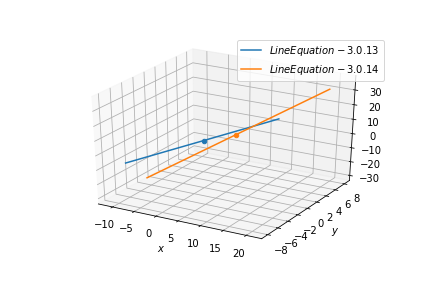
\includegraphics[width=\columnwidth]{./solutions/line_plane/74/codes/figs/Line_interest_2.png}
	\caption{Graph for equations \ref{eq:solutions/line_plane/74/codes14}}
	\label{fig:solutions/line_plane/74/codesline_equation_2}
\end{figure}
\end{enumerate}

    


\section{CONICS EXERCISE}
\subsection{Problem}
Sketch the circles with
\begin{align}
\brak{a}centre \myvec{0\\2}, radius 2
\\
\brak{b}centre \myvec{-2\\32}, radius 4
\\
\brak{c}centre \myvec{\frac{1}{2}\\\frac{1}{4}}, radius \frac{1}{12}
\\
\brak{d}centre \myvec{1\\1}, radius \sqrt{2}
\\
\brak{e}centre \myvec{-a\\-b}, radius \sqrt{a^2-b^2}
\end{align}

\subsection{Solution}
From theory, we understand that using dot product we can find the angle between the lines 
\begin{enumerate}
	\item 
	\begin{align}\label{eq:solutions/line_plane/74/codes:5}
		\frac{x-2}{2} = \frac{y-1}{5} &= \frac{z+3}{-3}, 
	\end{align}
	\begin{align}\label{eq:solutions/line_plane/74/codes:6}
		\frac{x+2}{-1} = \frac{y-4}{8} &= \frac{z-5}{4} 
	\end{align}


The above symmetric equations \ref{eq:solutions/line_plane/74/codes:5}, \ref{eq:solutions/line_plane/74/codes:6} can be represented in the vector form as 
\begin{align}\label{eq:solutions/line_plane/74/codes7}
	\quad \vec{r_1} &= \myvec{2\\1\\-3} + \lambda_1\myvec{2\\5\\-3}
	\\
	\quad \vec{r_2} &= \myvec{-2\\4\\5} + \lambda_2\myvec{-1\\8\\4}
\end{align}

As we have to find the angle between the vectors, we will only be taking the direction vectors into consideration. The direction vectors are $\vec{u}$ = $\myvec{2\\5\\-3}$ and $\vec{v}$ = $\myvec{-1\\8\\4}$. We can find the corresponding magnitude values

\begin{align}\label{eq:solutions/line_plane/74/codes9}
	\norm{\vec{u}} =\sqrt{2^{2}+5^{2}+(-3)^{2}} =\sqrt{38}
\end{align}
\begin{align}\label{eq:solutions/line_plane/74/codes10}
	\norm{\vec{v}} =\sqrt{(-1)^{2}+8^{2}+4^{2}} =\sqrt{81}
\end{align}

Using \ref{eq:solutions/line_plane/74/codes4}, \ref{eq:solutions/line_plane/74/codes9}, \ref{eq:solutions/line_plane/74/codes10} we get
\begin{align}
	\theta = \cos ^{-1}\frac{\myvec{2\\5\\-3}^{T}\myvec{-1\\8\\4}}{(\sqrt{38})(\sqrt{81})} 
	\\
	\theta = \cos ^{-1}\frac{26}{55.4797}
	\\
	\theta = \cos ^{-1} (0.4686)
	\\
	\theta = 62.053\degree
\end{align}

Therefore, the angle between the two lines is $62.053\degree$.See Fig. \ref{fig:solutions/line_plane/74/codesline_equation_1}

\begin{figure}
	\centering
	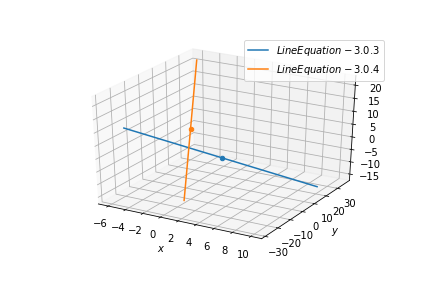
\includegraphics[width=\columnwidth]{./solutions/line_plane/74/codes/figs/Line_interest_1.png}
	\caption{Graph for equations \ref{eq:solutions/line_plane/74/codes7}}
	\label{fig:solutions/line_plane/74/codesline_equation_1}
\end{figure}


	\item 
	\begin{align}\label{eq:solutions/line_plane/74/codes12}
		\frac{x}{2} = \frac{y}{2} &= \frac{z}{1}, 
	\end{align}
	\begin{align}\label{eq:solutions/line_plane/74/codes13}
		\frac{x-5}{4} = \frac{y-2}{1} &= \frac{z-3}{8} 
	\end{align}



The above symmetric equations \ref{eq:solutions/line_plane/74/codes12}, \ref{eq:solutions/line_plane/74/codes13} can be represented in the vector form as 
\begin{align}\label{eq:solutions/line_plane/74/codes14}
	\quad \vec{r_1} &= \myvec{0\\0\\0} + \lambda_1\myvec{2\\2\\1}
	\\
	\quad \vec{r_2} &= \myvec{5\\2\\3} + \lambda_2\myvec{4\\1\\8}
\end{align}

As we have to find the angle between the vectors, we will only be taking the direction vectors into consideration. The direction vectors are $\vec{u}$ = $\myvec{2\\2\\1}$ and $\vec{v}$ = $\myvec{4\\1\\8}$. We can find the corresponding magnitude values

\begin{align}\label{eq:solutions/line_plane/74/codes16}
	\norm{\vec{u}} =\sqrt{2^{2}+2^{2}+1^{2}} =\sqrt{9}
\end{align}
\begin{align}\label{eq:solutions/line_plane/74/codes17}
	\norm{\vec{v}} =\sqrt{4^{2}+1^{2}+8^{2}} =\sqrt{81}
\end{align}

Using \ref{eq:solutions/line_plane/74/codes4}, \ref{eq:solutions/line_plane/74/codes16}, \ref{eq:solutions/line_plane/74/codes17} we get
\begin{align}
	\theta = \cos ^{-1}\frac{\myvec{2\\2\\1}^{T}\myvec{4\\1\\8}}{(\sqrt{9})(\sqrt{81})} 
	\\
	\theta = \cos ^{-1}\frac{18}{27.00}
	\\
	\theta = \cos ^{-1} (0.667)
	\\
	\theta = 48.189\degree
\end{align}

Therefore, the angle between the two lines is $48.189\degree$. See Fig. \ref{fig:solutions/line_plane/74/codesline_equation_2}


\begin{figure}
	\centering
	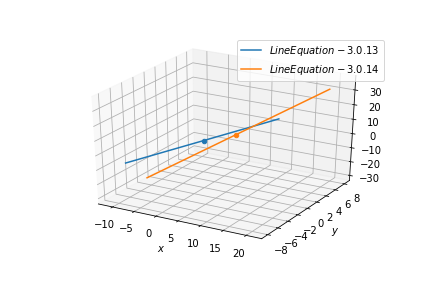
\includegraphics[width=\columnwidth]{./solutions/line_plane/74/codes/figs/Line_interest_2.png}
	\caption{Graph for equations \ref{eq:solutions/line_plane/74/codes14}}
	\label{fig:solutions/line_plane/74/codesline_equation_2}
\end{figure}
\end{enumerate}

    


\end{document}

